\subsection{Train Custom Data: Weights, Biases Logging, Local Logging}

\begin{figure}[t]
    \centerline{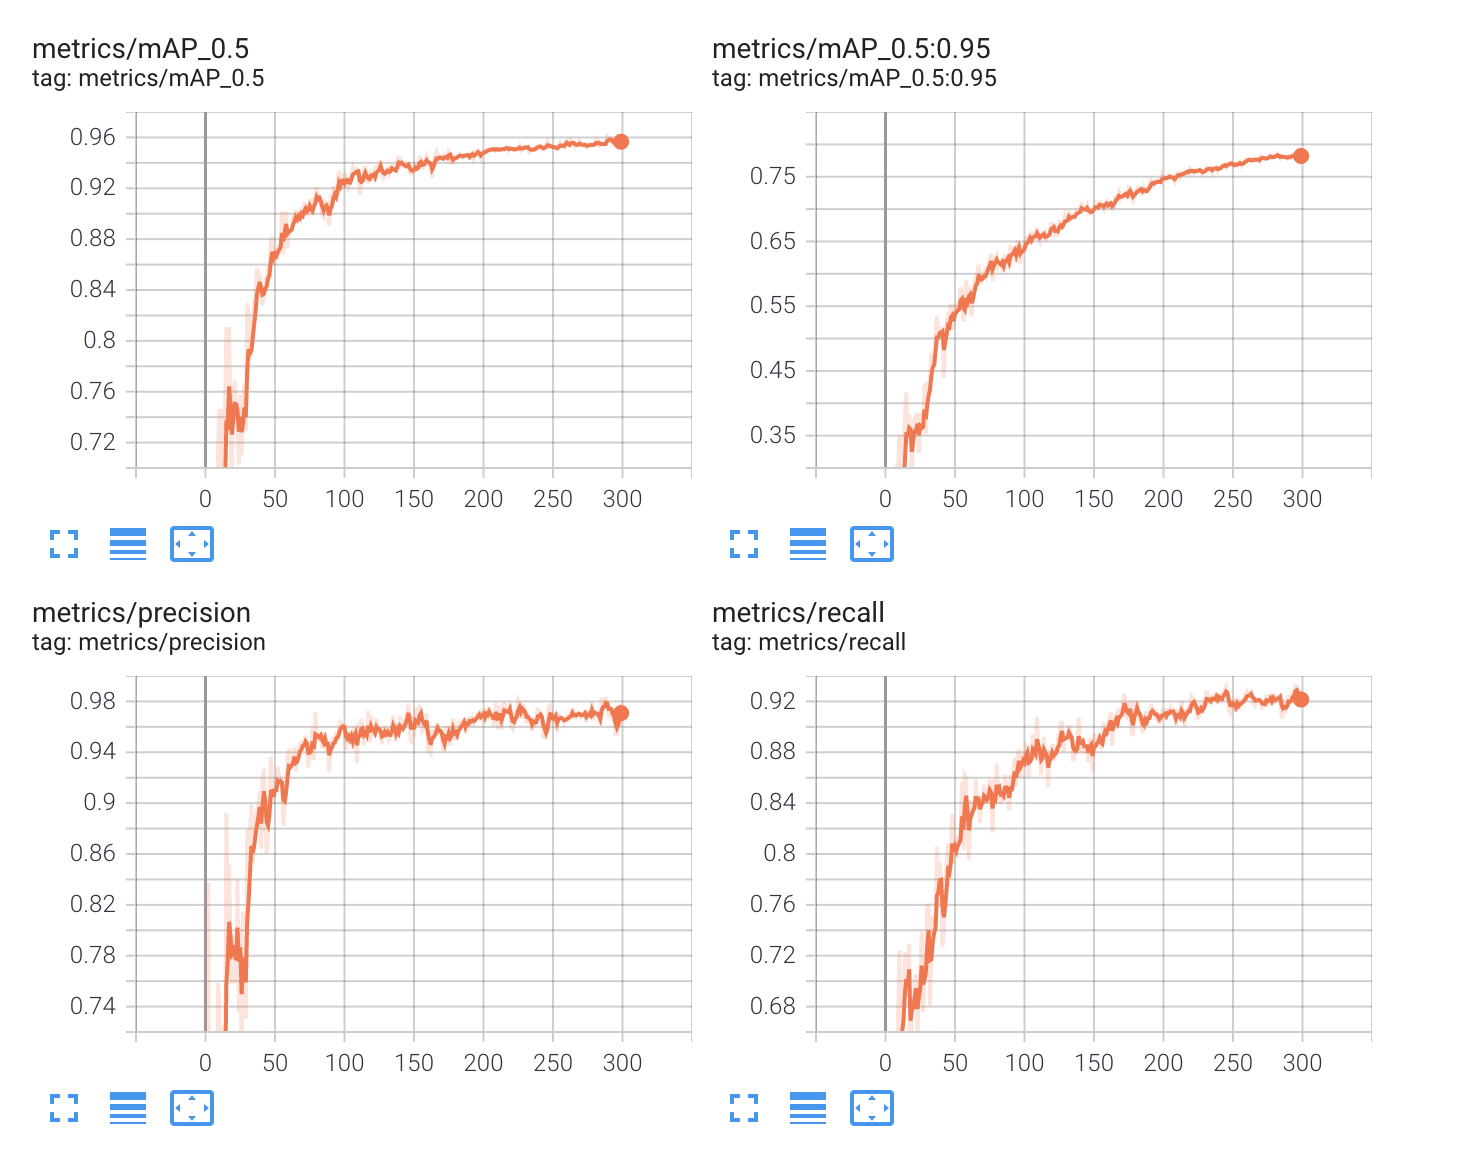
\includegraphics[width=\columnwidth]{img/colab_metrics.png}}
    \caption{Average model precision when IOU is larger than 0.5; Average model precision when IOU is between 0.5 and 0.95; The model precision; The model recall rate.}
    \label{fig:colab_metrics}
\end{figure}

\begin{figure}[t]
    \centerline{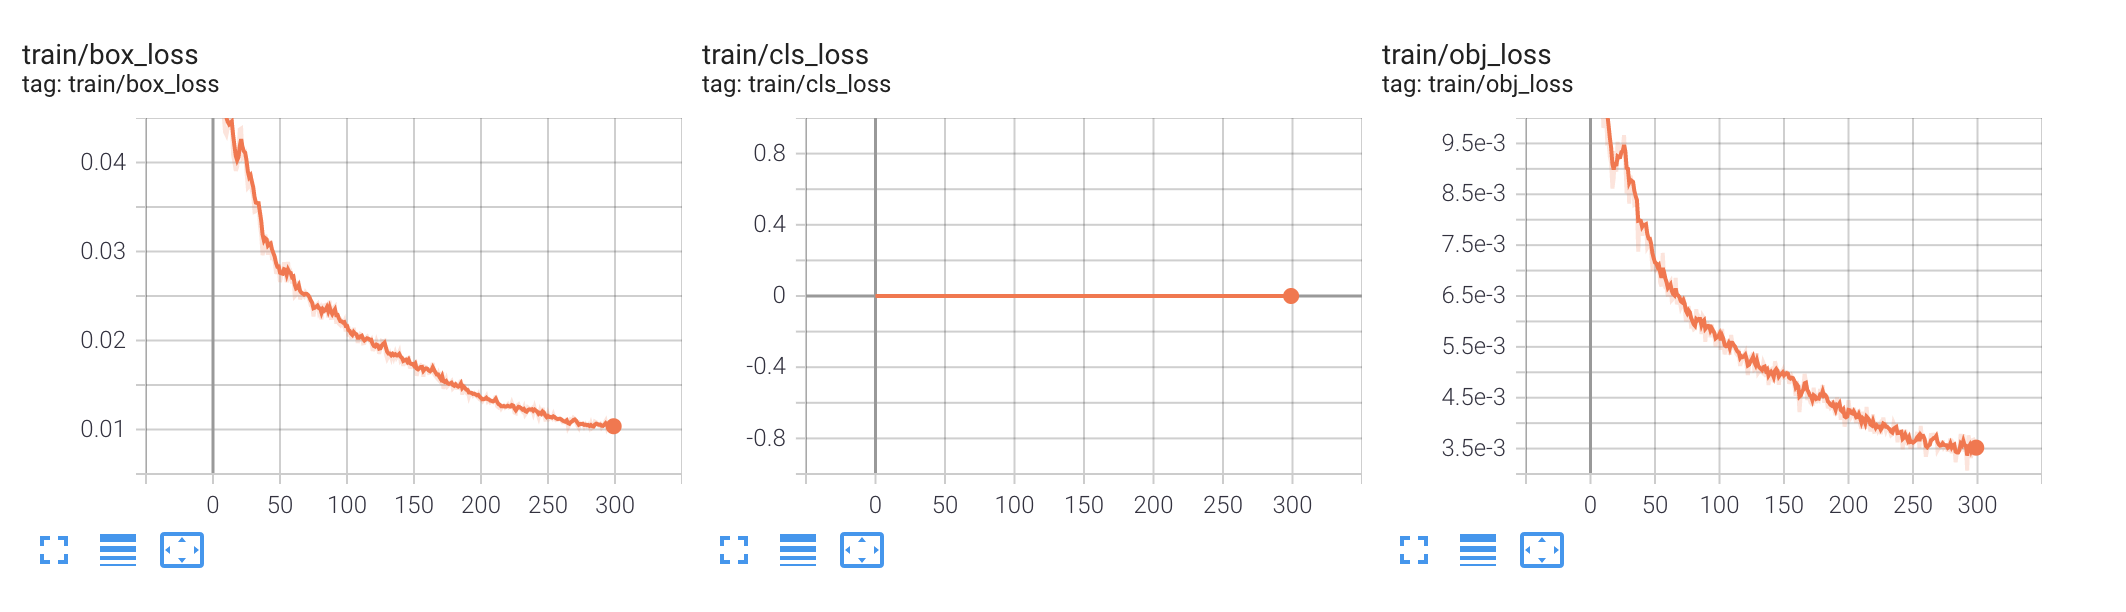
\includegraphics[width=\columnwidth]{img/colab_train.png}}
    \caption{The box loss rate of the model; The class loss rate of the model; The object loss rate of the model.}
    \label{fig:colab_train}
\end{figure}

\begin{figure}[t]
    \centerline{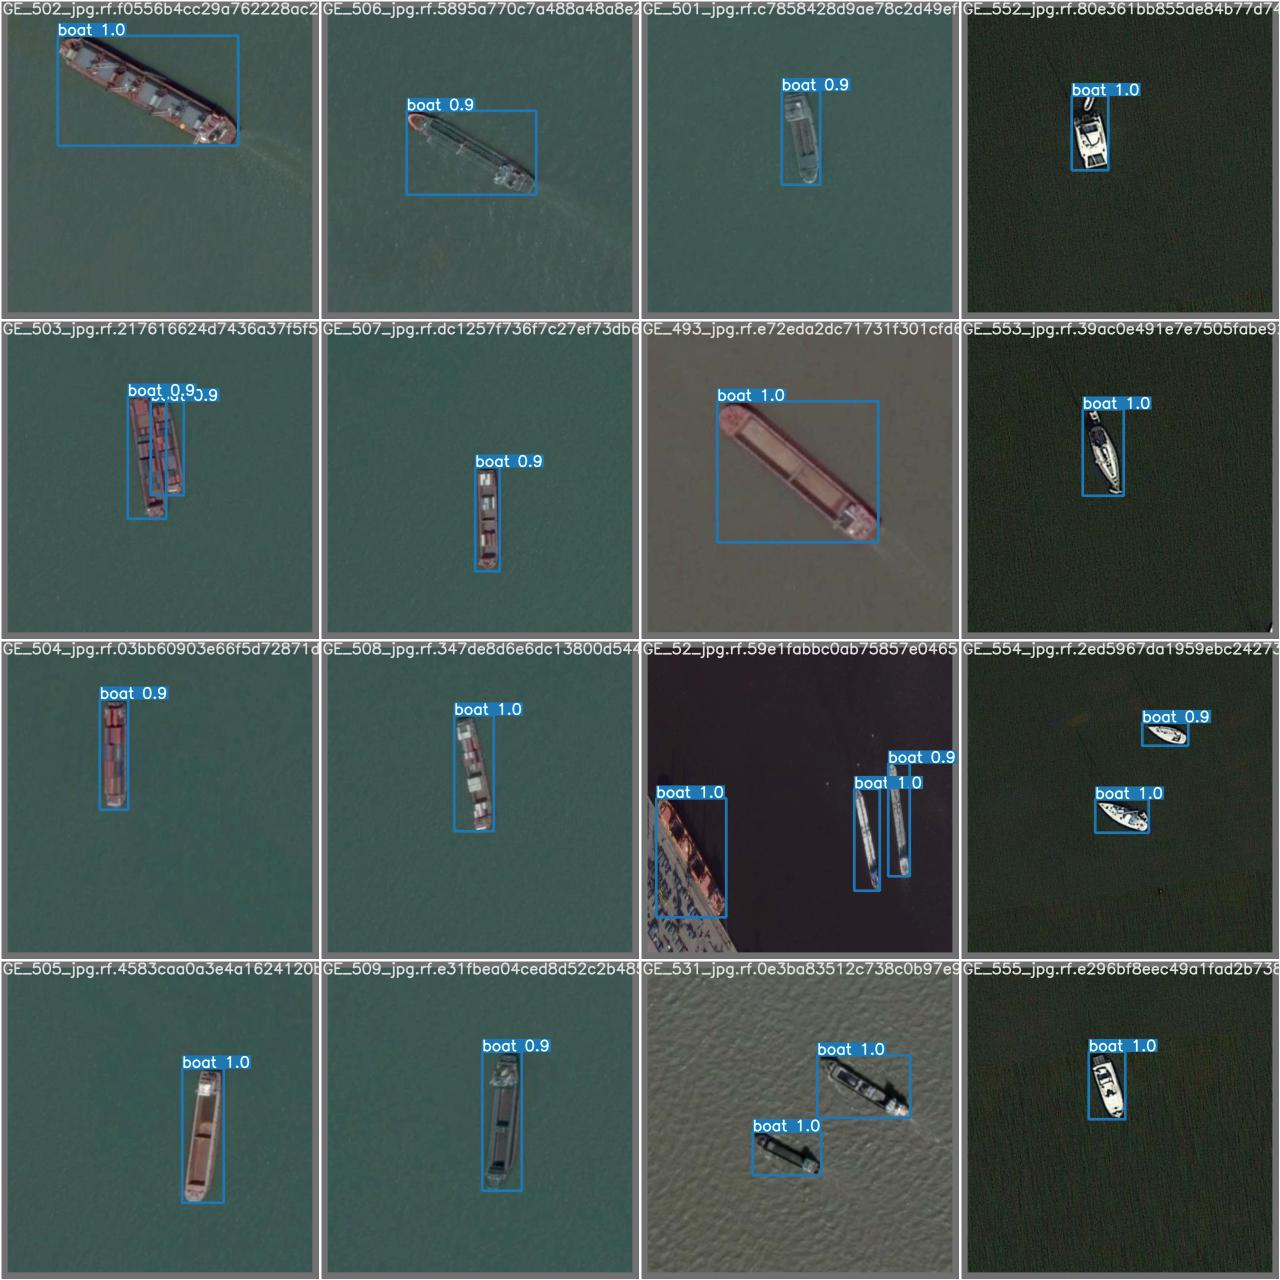
\includegraphics[width=\columnwidth]{img/test_batch1_pred.jpeg}}
    \caption{Test result of a trained model for detecting ships.}
    \label{fig:test_batch1_pred}
\end{figure}

As shown in Figure~\ref{fig:colab_metrics}, the average accuracy of the model, the precision of the model and the recall of the model all show a significant increase with the number of model training when the IOU\footnote{Intersection over Union is an evaluation metric used to measure the accuracy of an object detector on a particular dataset.} is between 50\% and 95\%. In particular, the precision of the model can eventually reach a level close to 96\%. However, this does not necessarily mean that the model will also fit satellite imagery of the Gulf of California. First, such high accuracy results only tell us that the model can achieve a relatively high recognition accuracy, which gradually increases and eventually reaches 96\% after 300 training repetitions. If the algorithm needs to be trained for this area, then consideration must be given to purposefully selecting many small boats in or near the area as a source of data for training the model. 

Secondly, there is also an inequity in the level of resolution of the training and test data. Each image from the Gulf of California was maintained at a resolution of 3840 pixels x 2160 pixels, which would result in the algorithm not framing the target perfectly when it detects it, i.e., it would not be perfectly tangential to the edges of the target.

To train models faster, we reduced the resolution of the images by a factor of about 70. Otherwise, the training could take half a month if used images with a resolution of 4800 pixels x 2908 pixels as the data source.

Similarly, as shown in Figure~\ref{fig:colab_train}, the loss rate of the box can eventually reach 1\% as the number of training sessions increases. Since this study has defined only one class of object, i.e. boat, this means that the probability that the detection box does not detect that it is a boat at all is 1\%. Similarly, because there is only one class, the class loss rate is 0. Figure~\ref{fig:test_batch1_pred} shows the prediction results during the training of the model, and it can be seen that the model can detect the presence of vessels in 100\% of the tested ranges and give the corresponding range boxes. Most of the detected boats have a 90\% probability of being boats, an acceptable value for object detection. Since only one class was set, some were also considered a 100\% probability of being boats.

\subsection{Detection Results and Small Boat Composition}
The error between the two approaches fall within an acceptable error range. In this section, the length measurement of the model is tested and compared against Google Earth Pro measuring tools for one small boat and a large ship. This will allow for the assessment of the algorithm precision. The results from Figure~\ref{fig:length_test} consistency that a small boat detected by the model measured 6.98 meters using Google Earth Pro measuring tools, while this work algorithm detected a length of 6.74 meters. The error between them is 3.44\%. With the larger boat Google Earth Pro measured 41.38 meters in length, and the algorithm detected 40.98 meters. The error between them is less than 1\%.

\begin{figure}[t]
    \center
    \includegraphics[width=\columnwidth]{img/length_test.png}
    \caption{Compare the length of boats with the use of Google Earth ruler and computer vision algorithm. It is the image from Google Earth Pro for Zurich Lake on 16th August 2018 when eye alt is 200 meters.}
    \label{fig:length_test}
\end{figure}

As explained in Sec~\ref{III-D-Detection-Architecture}, it was unproductive for the model to select the entire region for the study due to the varying amount of data that Google Earth Pro has been publicly available for the Gulf of California over the past three years. Therefore, three areas with more data were chosen: Santa Rosalia, Loreto, and Guaymas. Ultimately, satellite images of these three areas were found for 2019, 2020, and 2021, for a total of 690 images.

However, as stated in Sec~\ref{III-D-Detection-Architecture}, some of the slightly earlier satellite images had inferior detail representation capabilities, which resulted in the model not being very good at accurately detecting the features of the target, so that many small boats in the Gulf of California could not be detected. To improve the model accuracy, it was used an image enhancement process with a 5x5 sharpening kernel, achieving a higher recognition rate. However, the following situations still occur.

\begin{enumerate}
    \item Figure~\ref{fig:1_docked_together_Guaymas_202001_20}: When the detailed representation of the image is indigent, and two or three small boats are moored together, the model is very likely to recognize the two or three boats as a whole. There are two reasons for this problem. First, the training data is primarily a `fuzzy' data source. Thus, when there are two or three small boats moored together, the model cannot easily detect the features of each small boat individually. In contrast, it may seem more reasonable to the model that the two or three boats as a whole have the same features. The second reason is that most data sources are individual boats on the surface or boats docked close to each other. As the data sources do not fully consider the fuzzy nature of the detail needed to detect the object and the fact that they are too close together, the model naturally does not recognize such cases.
    
    \item Figure~\ref{fig:2_square_Guaymas_202001_01}: When a large cargo ship is moored, the ship appears as a 'rectangle' from the air, much like a long pier, and is sometimes undetectable because small vessels with a rectangular shape were not common at the time data feed was compiled. This also applies to uncommon vessels such as battleships. This could be corrected if the model considered larger ships but this was outside the scope of this work.

    \item Figure~\ref{fig:3_beach_SantaRosalia_202104_02}: The recognition rate was also significantly lower when the boats were sometimes laying on the beach rather than floating on the water This is because most of the training data is based images that contained on the water rather than the boats on the beach.

\end{enumerate}

\begin{figure}[t]
    \centering
    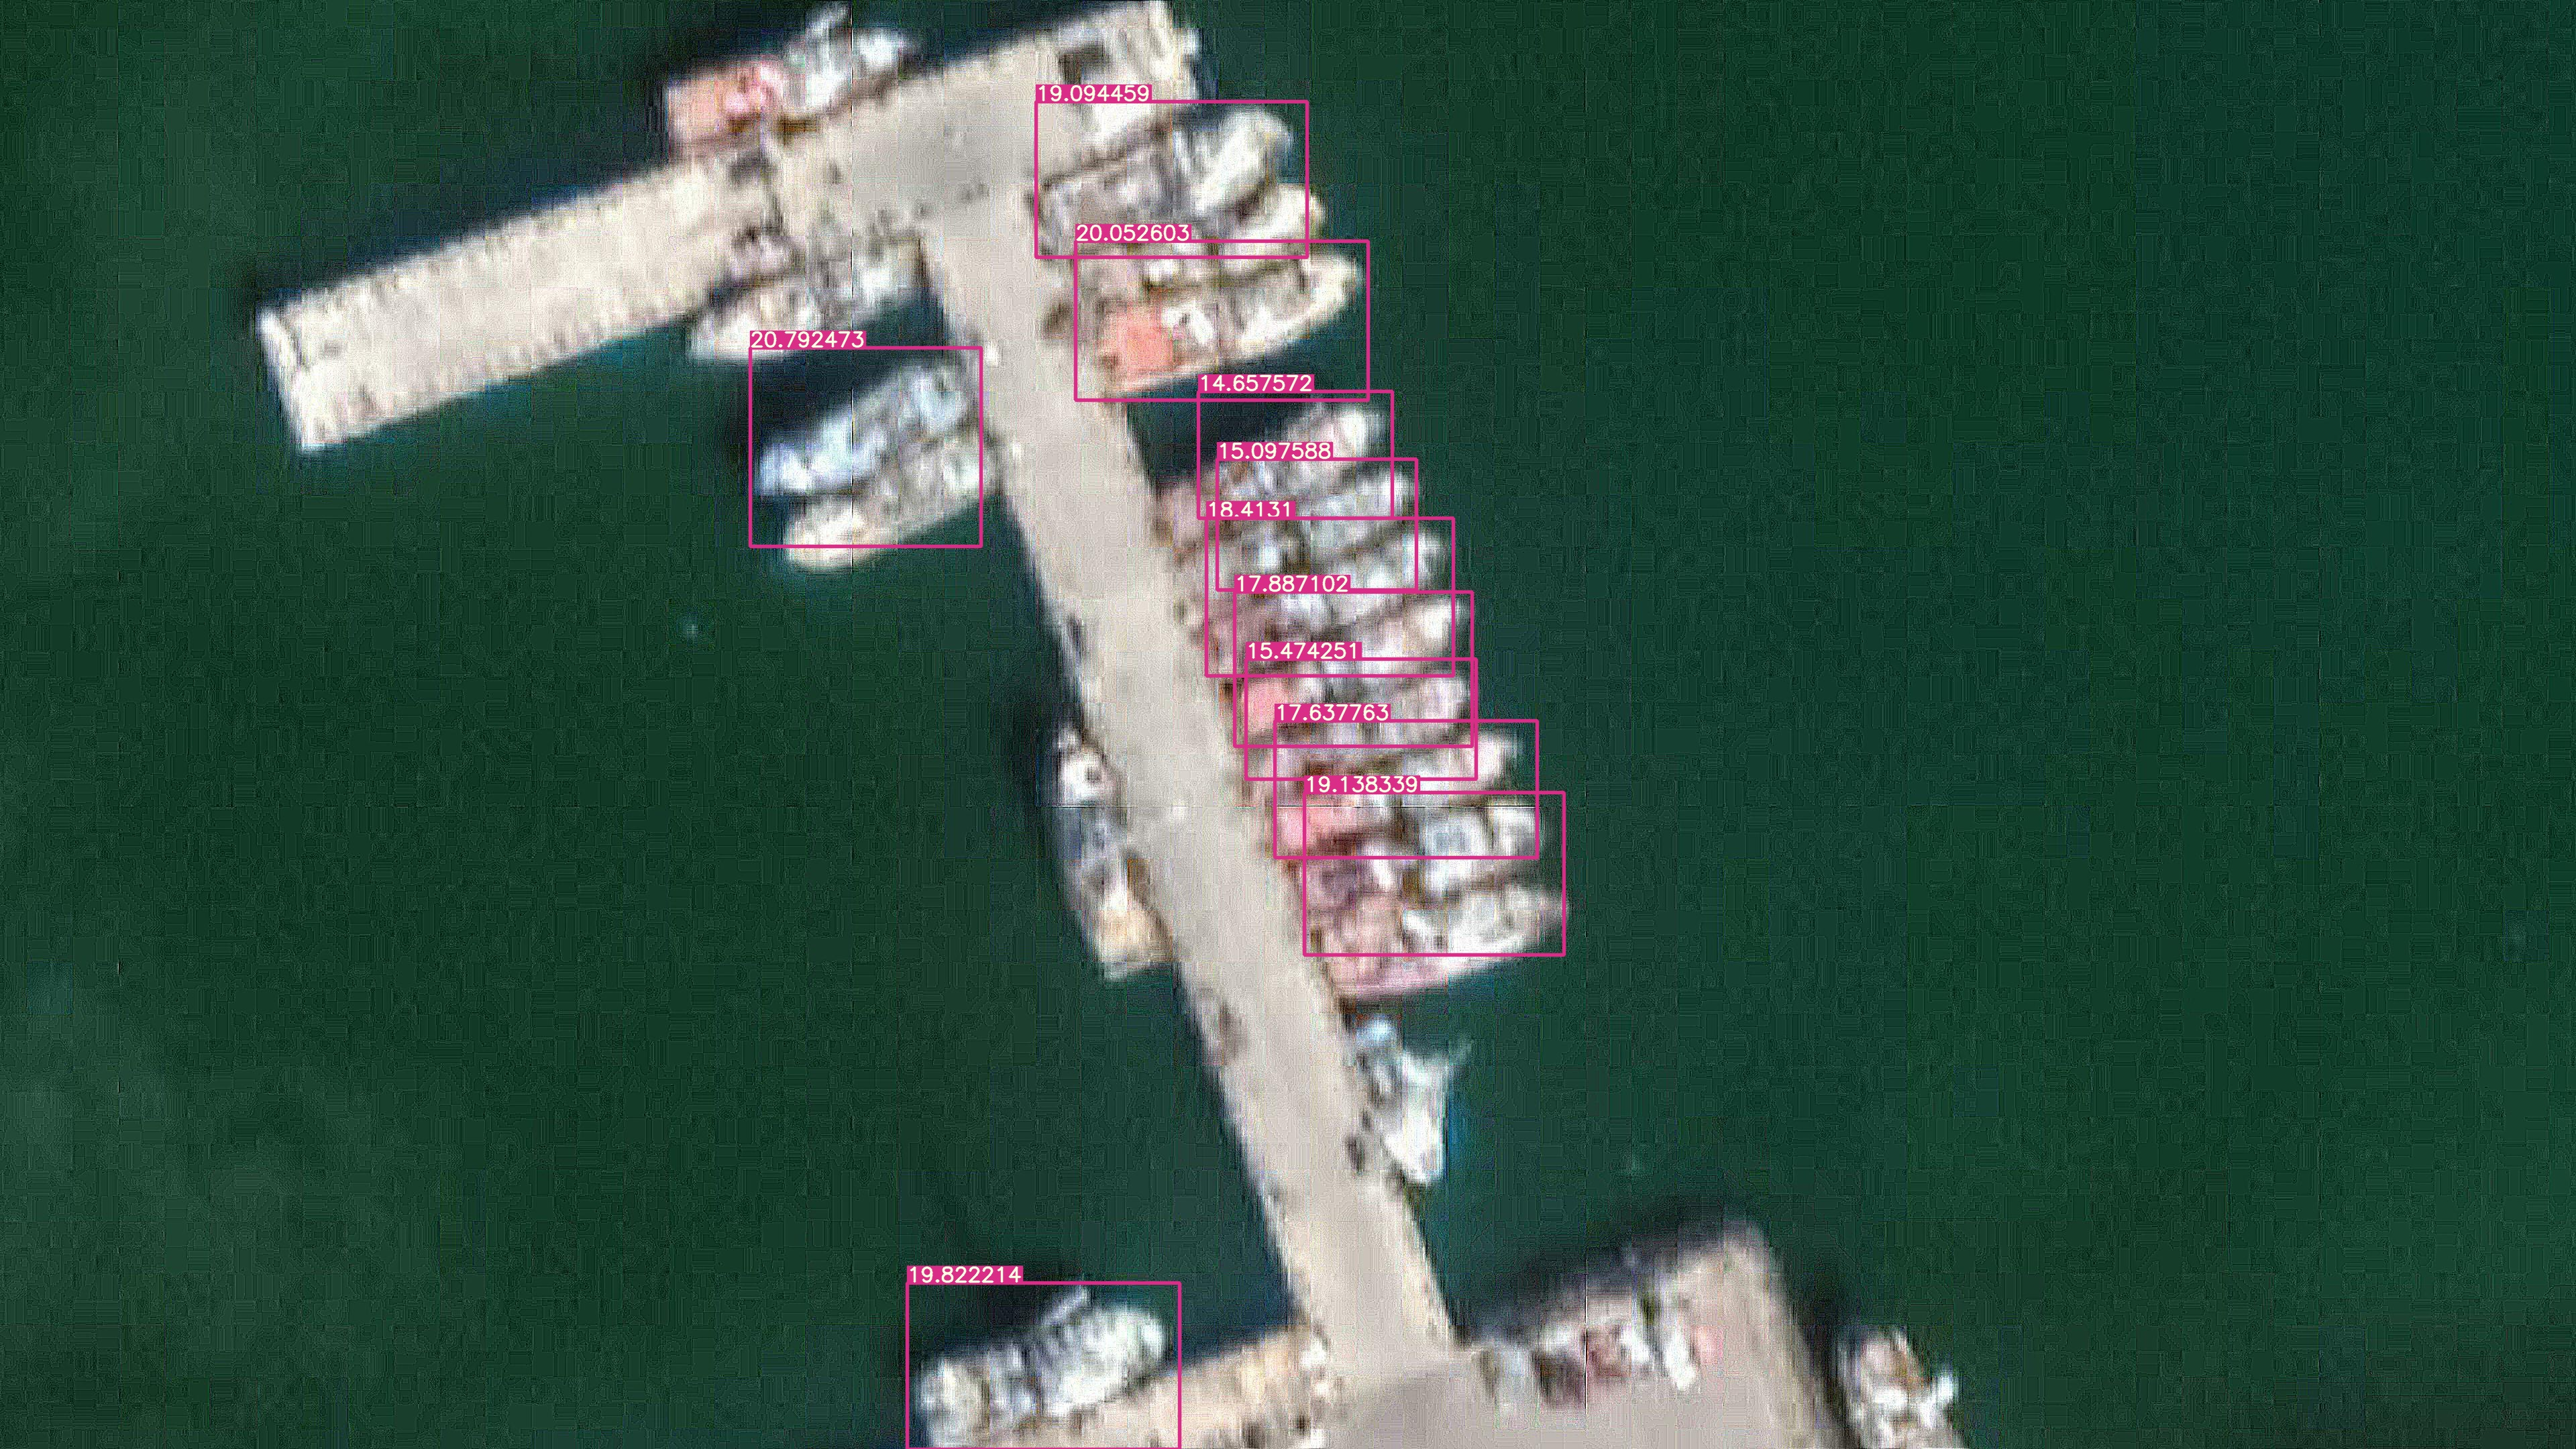
\includegraphics[width=\columnwidth]{img/1_docked_together_Guaymas_202001_20.jpeg}
    \caption{When small boats are moored closely together in the harbor, the model may recognize two small boats as one. Image is from Guaymas, Janurary 2020.}
    \label{fig:1_docked_together_Guaymas_202001_20}
\end{figure}

\begin{figure}[t]
    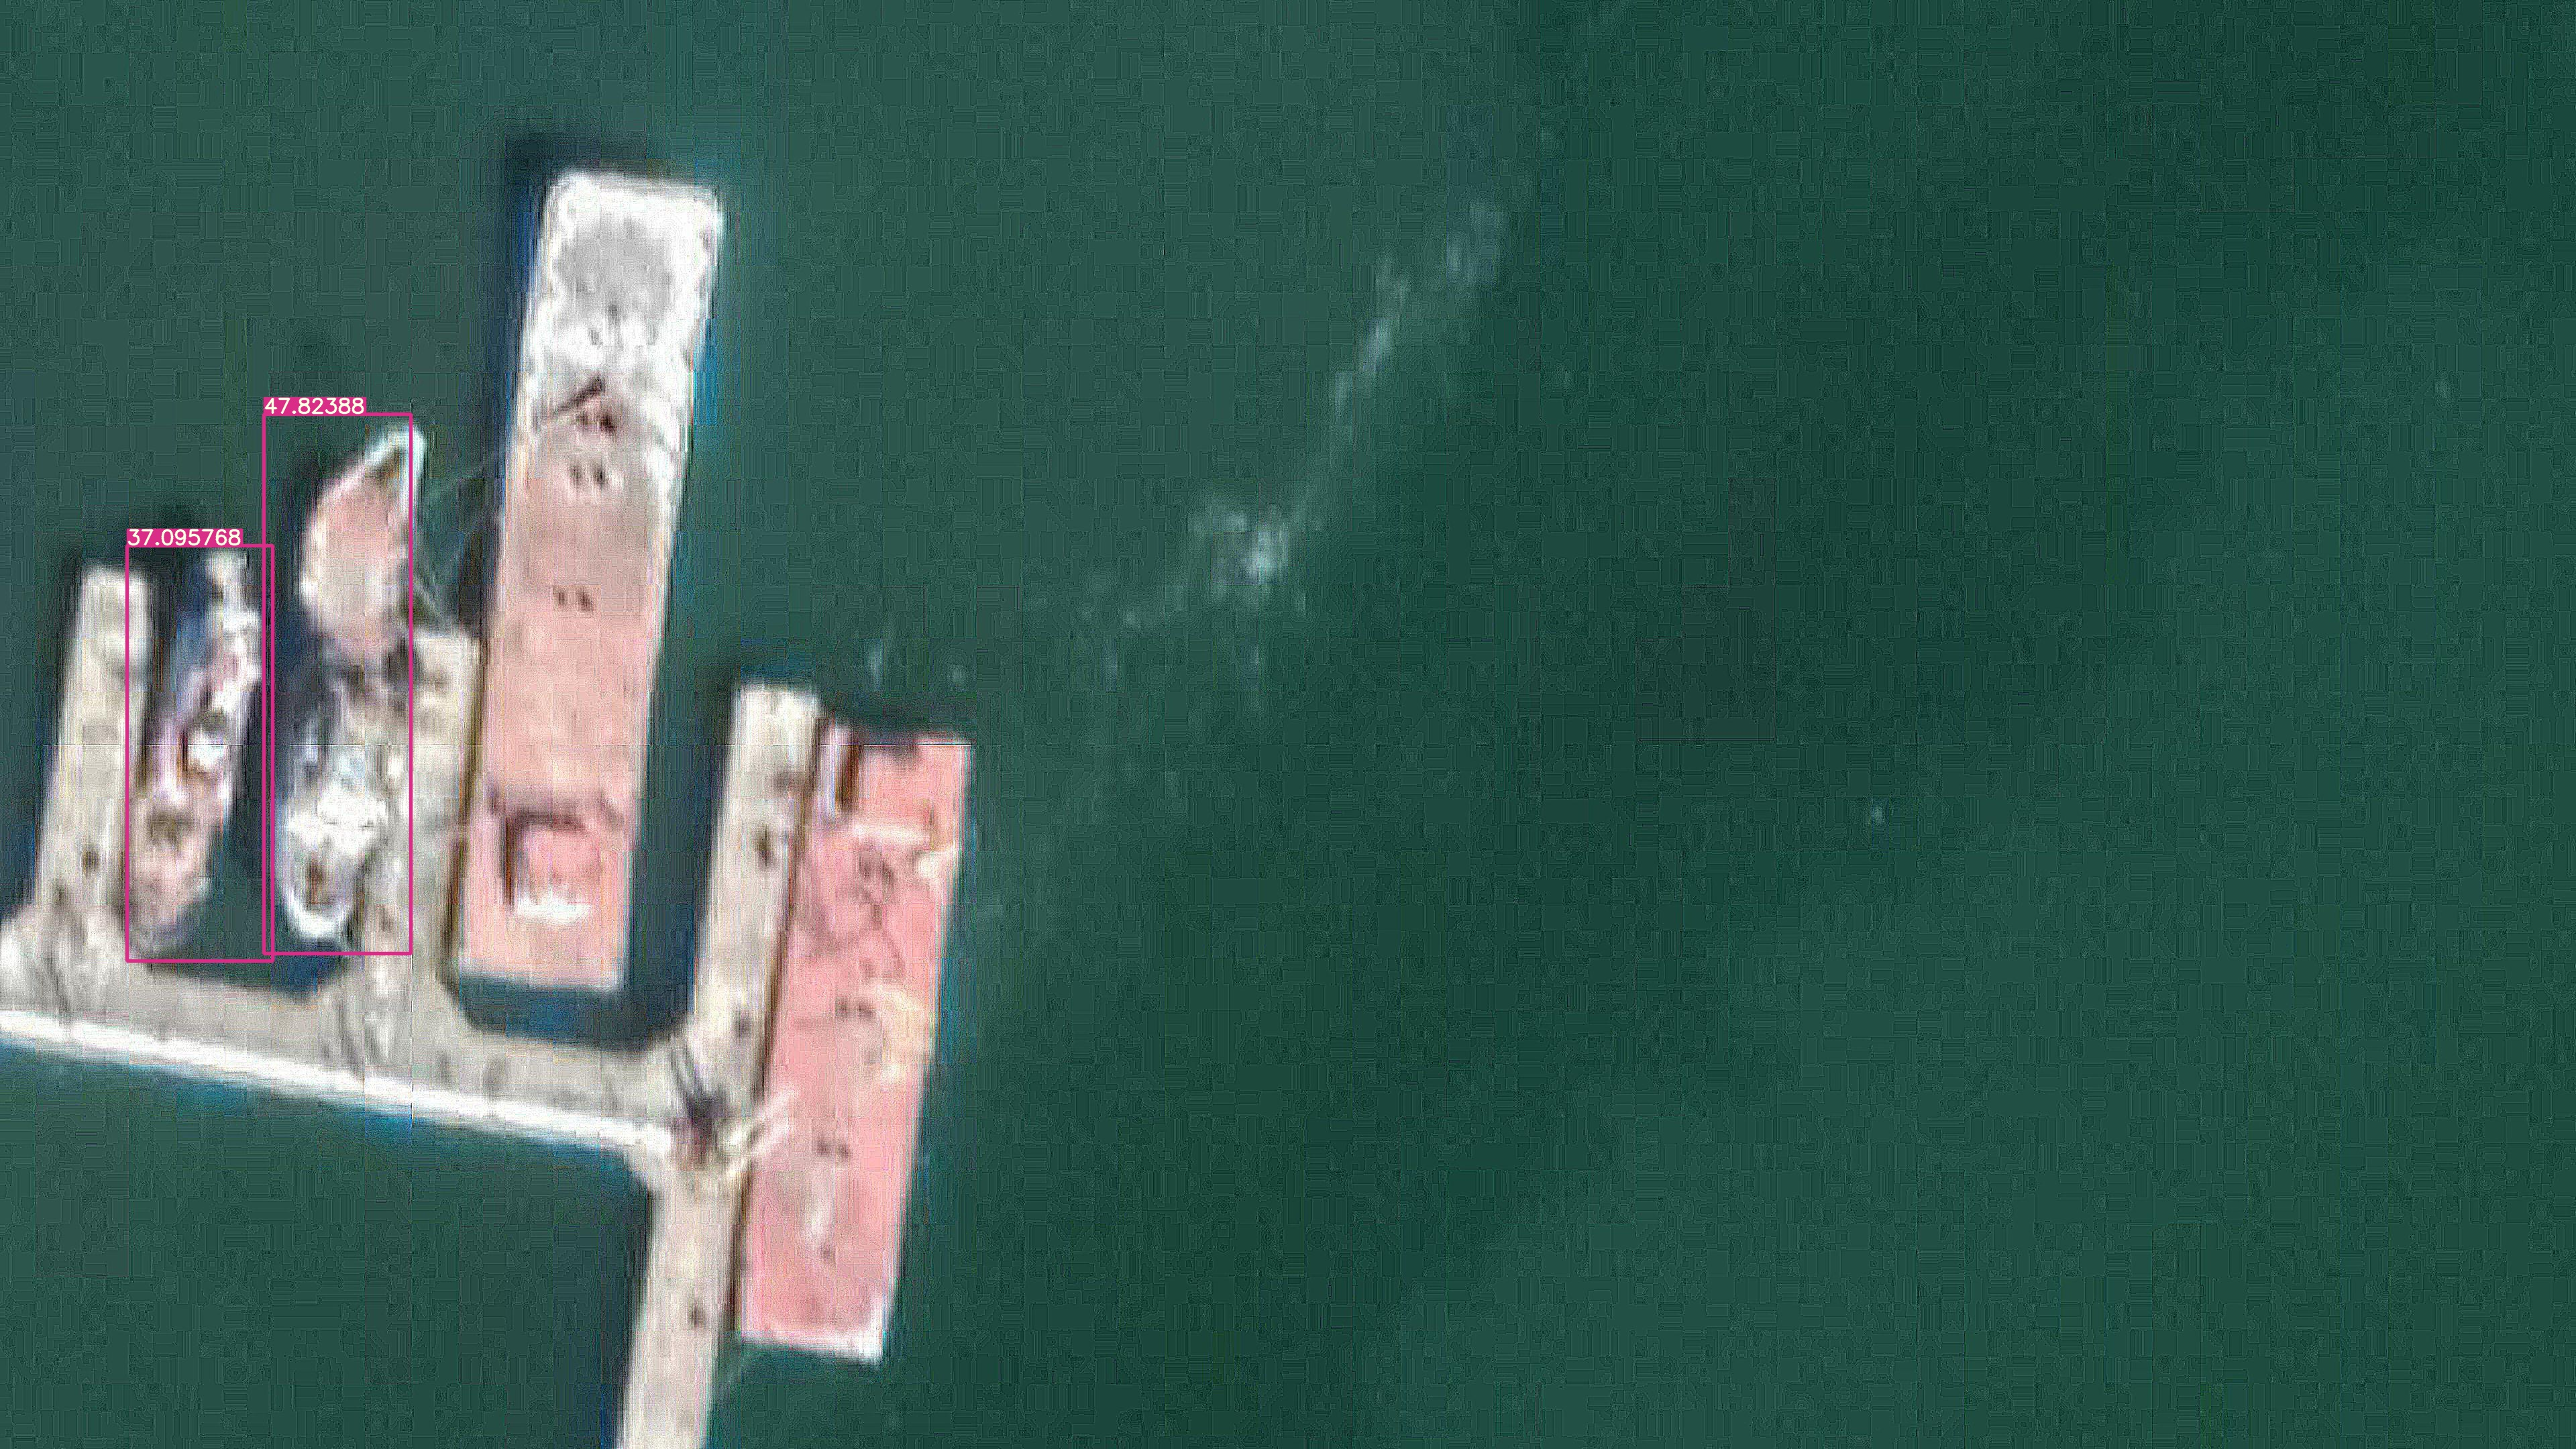
\includegraphics[width=\columnwidth]{img/2_square_Guaymas_202001_01.jpeg}
    \caption{When the cargo ship is full of cargo, the ship looks like a rectangular jetty from above and loses the normal shape of a ship. Image is from Guaymas, Janurary 2020.}
    \label{fig:2_square_Guaymas_202001_01}
\end{figure}

\begin{figure}[t]
    \includegraphics[width=\columnwidth]{img/3_beach_SantaRosalia_202104_02.jpeg}
    \caption{Models may have difficulty detecting small boats moored on the beach. Image is from Santa Rosalia, February 2021.}
    \label{fig:3_beach_SantaRosalia_202104_02}
\end{figure}



\begin{figure}[t]
    \center
    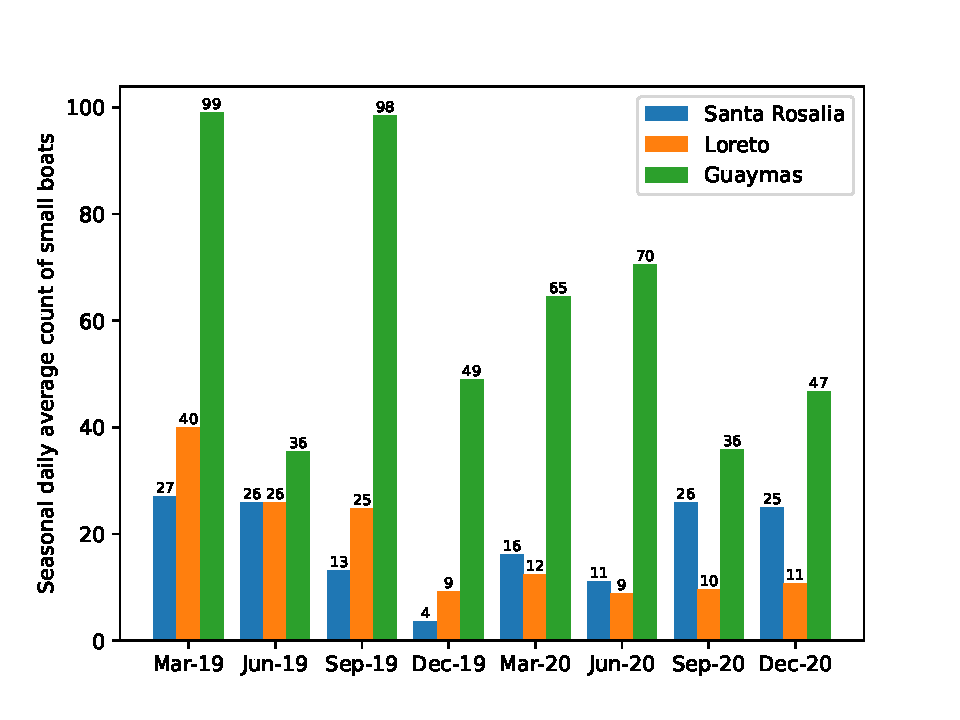
\includegraphics[width=\columnwidth]{img/avg_small.pdf}
    \caption{Seasonal daily average count of small boats in Santa Rosalia, Loreto, and Guaymas between 2019 and 2020.}
    \label{fig:avg_small}

    \center
    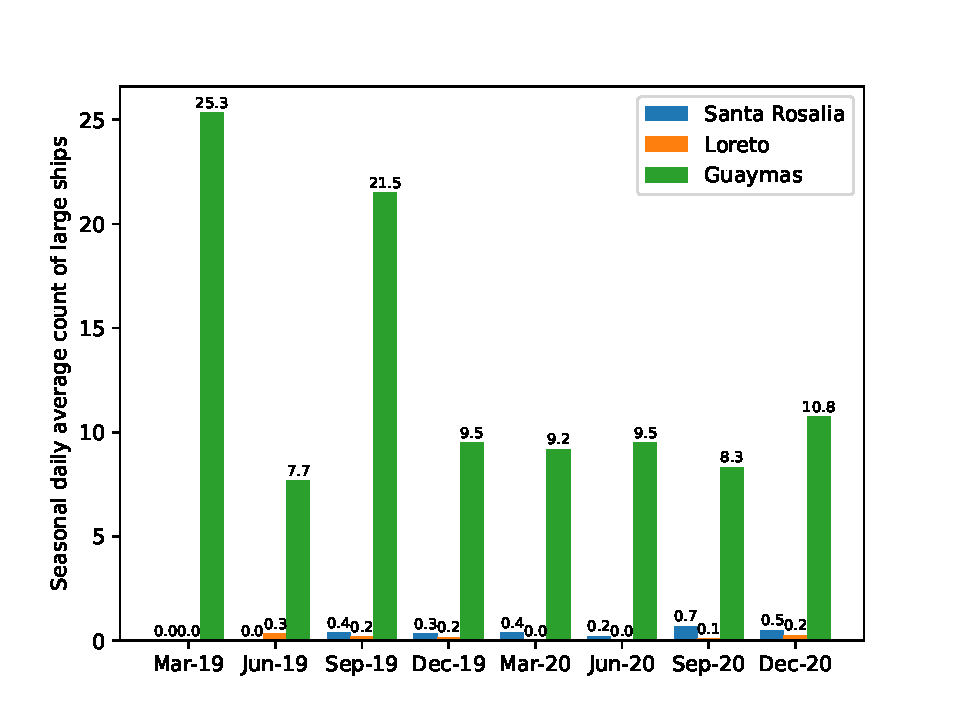
\includegraphics[width=\columnwidth]{img/avg_big.pdf}
    \caption{Seasonal daily average count of large ships in Santa Rosalia, Loreto, and Guaymas between 2019 and 2020.}
    \label{fig:avg_big}
\end{figure}

Nevertheless, as Figures~\ref{fig:1_docked_together_Guaymas_202001_20},~\ref{fig:2_square_Guaymas_202001_01},~\ref{fig:3_beach_SantaRosalia_202104_02} demonstrate, the model still detects most of the small boats in poorly detailed satellite images, even those images that human eyes cannot easily detect. The number of small and large ships between regions can be seen in Figure~\ref{fig:avg_small} and Figure~\ref{fig:avg_big}. Guaymas, Loreto and Santa Rosalia can be classed by two different types of port cities:

\begin{enumerate}
    \item Santa Rosalia and Loreto have a much smaller number of small boats and almost no large ships.
    \item The port of Guaymas presented a larger number of small boats when contrasted to the other two coastal cities. There was between 1.37 and 8.00 times more small boats detected in Guaymas than in Santa Rosalia (dependent on the month and year of the image) and 3.00 times more than in Loreto. 
    \item Guaymas had a larger number of large ships as well. There was more than 10 times more large ships detected in Guaymas than in Santa Rosalia and in Loreto.
    \item In the relatively large seaports of Guaymas and Loreto, there is a tendency for both large and small vessels to decrease with time.
\end{enumerate}

In fact, according to statistic\cite{INEGI2022Population} from Mexican government, in 2020, the population of Guaymas, Loreto, and Santa Rosalia are 156,863, 18,052, and 14,357 separately. It will seem that the number of detected boats is correlated to the number of habitants which makes sense since by probability there would be more economic and leisure activities around Guaymas.


\subsection{Entertainment and Fishing Boats in the Gulf of California}



\begin{table}[t]
\center
\begin{tabular}{|c|c|c|c|c|}
\hline
                                &  Mar-20   & Jun-20    & Sep-20    & Dec-20\\ \hline
   Small boats                  &  323      & 283       & 215       & 187   \\ \hline
   Large ships                  &  46       & 38        & 50        & 43    \\ \hline
   Small white boats            &  302      & 273       & 210       & 174   \\ \hline
\end{tabular}
\caption{\textbf{Detection example.} Small boats, large ships, and small white boats in Guaymas in 2020.}
\label{Guaymas_2020}
\end{table}

According to the statement in Sec~\ref{III-D-Detection-Architecture}, determining whether a boat is white or not can be used as a criterion to determine whether a boat for recreation or for fishing. As can be seen from Table~\ref{Guaymas_2020}, most of the small boats in Guaymas in 2020 are white, i.e., all can be classified as recreational boats. However, as discussed before, this conclusion is limited since the algorithm does not consider, for example, other colors as part of the leisure boats. Although there are many uncertainties in detecting the color of the boats, the algorithm also takes into account situations where the color of the boats is not fully white due to atmospheric refraction, weather conditions, or cloud interference. This means that the algorithm also takes into account situations where the color of the boats is light. This approach is acceptable from the point of view of algorithm complexity, results, and detecting data quality.